%% Преамбула TeX-файла

% 1. Стиль и язык
\documentclass[utf8x, times, 14pt]{G7-32} % Стиль (по умолчанию будет 14pt)
\bibliographystyle{gost780u}

% Остальные стандартные настройки убраны в preamble.inc.tex.
\sloppy

% Настройки стиля ГОСТ 7-32
% Для начала определяем, хотим мы или нет, чтобы рисунки и таблицы нумеровались в пределах раздела, или нам нужна сквозная нумерация.
\EqInChapter % формулы будут нумероваться в пределах раздела
\TableInChapter % таблицы будут нумероваться в пределах раздела
\PicInChapter % рисунки будут нумероваться в пределах раздела

% Добавляем гипертекстовое оглавление в PDF
\usepackage[
bookmarks=true, colorlinks=true, unicode=true,
urlcolor=black,linkcolor=black, anchorcolor=black,
citecolor=black, menucolor=black, filecolor=black,
]{hyperref}

\AfterHyperrefFix

\usepackage{microtype}% полезный пакет для микротипографии, увы под xelatex мало чего умеет, но под pdflatex хорошо улучшает читаемость

% Тире могут быть невидимы в Adobe Reader
\ifInvisibleDashes
\MakeDashesBold
\fi


\usepackage{graphicx}   % Пакет для включения рисунков

% С такими оно полями оно работает по-умолчанию:
% \RequirePackage[left=20mm,right=10mm,top=20mm,bottom=20mm,headsep=0pt,includefoot]{geometry}
% Если вас тошнит от поля в 10мм --- увеличивайте до 20-ти, ну и про переплёт не забывайте:
\geometry{right=20mm}
\geometry{left=30mm}
\geometry{bottom=20mm}
\geometry{ignorefoot}% считать от нижней границы текста

\usepackage{rotating}

% доп. позиционирование таблиц
\usepackage{float}

% таблицы с автоматическим определением ширины
\usepackage{tabularx}

% для ультра лютой большой таблицы
\usepackage{xltabular}

% Пакет Tikz
\usepackage{tikz}
\usetikzlibrary{arrows,positioning,shadows}

% Произвольная нумерация списков.
\usepackage{enumerate}

% ячейки в несколько строчек
\usepackage{multirow}

% itemize внутри tabular
\usepackage{paralist,array}
\newcolumntype{Y}{>{\centering\arraybackslash}X}

%\setlength{\parskip}{1ex plus0.5ex minus0.5ex} % разрыв между абзацами
\setlength{\parskip}{1ex} % разрыв между абзацами
\setlength{\intextsep}{4pt}
\setlength{\abovecaptionskip}{4pt}
\setlength{\floatsep}{5pt plus 1.0pt minus 1.0pt}
\usepackage{blindtext}

% Центрирование подписей к плавающим окружениям
%\usepackage[justification=centering]{caption}

\usepackage{newfloat}
\DeclareFloatingEnvironment[
placement={!ht},
name=Equation
]{eqndescNoIndent}
\edef\fixEqndesc{\noexpand\setlength{\noexpand\parindent}{\the\parindent}\noexpand\setlength{\noexpand\parskip}{\the\parskip}}
\newenvironment{eqndesc}[1][!ht]{%
    \begin{eqndescNoIndent}[#1]%
\fixEqndesc%
}
{\end{eqndescNoIndent}}

% Настройки листингов.
\ifPDFTeX
% 8 Листинги

\usepackage{listings}

% Значения по умолчанию
\lstset{
  basicstyle= \footnotesize,
  breakatwhitespace=true,% разрыв строк только на whitespacce
  breaklines=true,       % переносить длинные строки
%   captionpos=b,          % подписи снизу -- вроде не надо
  inputencoding=koi8-r,
  numbers=left,          % нумерация слева
  numberstyle=\footnotesize,
  showspaces=false,      % показывать пробелы подчеркиваниями -- идиотизм 70-х годов
  showstringspaces=false,
  showtabs=false,        % и табы тоже
  stepnumber=1,
  tabsize=4,              % кому нужны табы по 8 символов?
  frame=single
}

% Стиль для псевдокода: строчки обычно короткие, поэтому размер шрифта побольше
\lstdefinestyle{pseudocode}{
  basicstyle=\small,
  keywordstyle=\color{black}\bfseries\underbar,
  language=Pseudocode,
  numberstyle=\footnotesize,
  commentstyle=\footnotesize\it
}

% Стиль для обычного кода: маленький шрифт
\lstdefinestyle{realcode}{
  basicstyle=\scriptsize,
  numberstyle=\footnotesize
}

% Стиль для коротких кусков обычного кода: средний шрифт
\lstdefinestyle{simplecode}{
  basicstyle=\footnotesize,
  numberstyle=\footnotesize
}

% Стиль для BNF
\lstdefinestyle{grammar}{
  basicstyle=\footnotesize,
  numberstyle=\footnotesize,
  stringstyle=\bfseries\ttfamily,
  language=BNF
}

% Определим свой язык для написания псевдокодов на основе Python
\lstdefinelanguage[]{Pseudocode}[]{Python}{
  morekeywords={each,empty,wait,do},% ключевые слова добавлять сюда
  morecomment=[s]{\{}{\}},% комменты {а-ля Pascal} смотрятся нагляднее
  literate=% а сюда добавлять операторы, которые хотите отображать как мат. символы
    {->}{\ensuremath{$\rightarrow$}~}2%
    {<-}{\ensuremath{$\leftarrow$}~}2%
    {:=}{\ensuremath{$\leftarrow$}~}2%
    {<--}{\ensuremath{$\Longleftarrow$}~}2%
}[keywords,comments]

% Свой язык для задания грамматик в BNF
\lstdefinelanguage[]{BNF}[]{}{
  morekeywords={},
  morecomment=[s]{@}{@},
  morestring=[b]",%
  literate=%
    {->}{\ensuremath{$\rightarrow$}~}2%
    {*}{\ensuremath{$^*$}~}2%
    {+}{\ensuremath{$^+$}~}2%
    {|}{\ensuremath{$|$}~}2%
}[keywords,comments,strings]

% Подписи к листингам на русском языке.
\renewcommand\lstlistingname{Листинг}
\renewcommand\lstlistlistingname{Листинги}

\else
\usepackage{local-minted}
\fi

% Полезные макросы листингов.
%% Любимые команды
\newcommand{\Code}[1]{\textbf{#1}}

%\usepackage{unicode-math}
\DeclareMathOperator*{\Dap}{Δ P_c}

% Стиль титульного листа и заголовки
%\include{00-title}


\begin{document}

\frontmatter % выключает нумерацию ВСЕГО; здесь начинаются ненумерованные главы: реферат, введение, глоссарий, сокращения и прочее.

\maketitle %создает титульную страницу


%\begin{executors}
%\personalSignature{Первый исполнитель}{ФИО}
%
%\personalSignature{Второй исполнитель}{ФИО}
%\end{executors}


%\listoffigures                         % Список рисунков

%\listoftables                          % Список таблиц

%\NormRefs % Нормативные ссылки 
% Команды \breakingbeforechapters и \nonbreakingbeforechapters
% управляют разрывом страницы перед главами.
% По-умолчанию страница разрывается.

% \nobreakingbeforechapters
% \breakingbeforechapters

%% Также можно использовать \Referat, как в оригинале
\begin{abstract}

   Для электрической сети, схема которой показана на *, на основании исходных данных по узлам и ветвям, приведенных в табл. * и *:
   
   \begin{enumerate}[1.]
   	\item Составить схему замещения сети и определить ее параметры
   	\item Выполнить расчеты потокораспределения и напряжений в узлах сети в нормальном режиме наибольших нагрузок.
   	\item Выполнить расчеты потокораспределения и напряжений в узлах сети в нормальном режиме наименьших нагрузок.
   	\item Выполнить расчеты потокораспределения и напряжений в узлах сети в послеаварийном
   	режиме (отключение одной цепи линии).
   	\item Оценить достаточность регулировочных диапазонов устройств РПН трансформаторов на
   	подстанции.
   	\item Рассчитать потери активной мощности и годовые потери электроэнергии в сети.
   \end{enumerate}

\end{abstract}

%%% Local Variables: 
%%% mode: latex
%%% TeX-master: "rpz"
%%% End: 


\tableofcontents

%\printnomenclature % Автоматический список сокращений



\include{00-intro}

\mainmatter % это включает нумерацию глав и секций в документе ниже

\chapter{Характеристика исходных данных курсового проекта}
\label{cha:ish_dannie}

\newcolumntype{Z}{>{\centering\arraybackslash}X}

\section{Исходные данные для проектирования}

Электрическая сеть сооружается в Костромской области на железобетонных опорах.

\begin{figure}[h]
	\centering
	\includegraphics[width=0.7\textwidth]{inc/svg/scheme}
	\caption{Схема расположения пунктов}
	\label{fig:scheme}
\end{figure}

Питание района электроэнергией будет осуществляться от шин 220 кВ подстанции "К" работающей в составе электроэнергетической системы. Источник питания в режиме наибольших нагрузок обеспечивает полную выдачу необходимой для потребителей активной мощности, а также 87 Мвар реактивной мощности. На шинах источника питания района в режиме наибольших нагрузок обеспечивается напряжение, равно 110 \%, а в режиме наименьших нагрузок 100 \% от номинального.

Для всех пунктов наименьшая нагрузка принимается 37 \% от наибольшей; число часов использования наибольших нагрузок составляет \(4350\; \frac{\textup{ч}}{\textup{год}}\).

Вторичное напряжение на всех сооружаемых подстанциях 10 кВ.

\section{Исходные данные по климатическим условиям и нагрузкам в пунктах потребления}

Среднеянварская температура: \(-11,8\; ^oC\)

Среднегодовая температура: \(2,7\; ^oC\)

Среднеиюльская температура: \(17,6\; ^oC\)

Ветровой район: I

Район по гололёду: I

Определим коэффициент реактивной мощности нагрузки \(\tg \, \varphi_\textup{нб1}\), потребляемую реактивную мощность \(Q_\textup{нб1}\) и полную мощность \(S_\textup{нб1}\) для пункта 1:
\[\tg \, \varphi_\textup{нб1} = \tg(\arccos(\cos\, \varphi_\textup{нб1})) = \tg(\arccos(0,92)) = 0,426\]
\[Q_\textup{нб1} = P_\textup{нб1} \cdot \tg\, \varphi_\textup{нб1} = 70 \cdot 0,426 = 29,8\; \textup{Мвар}\]
\[S_\textup{нб1} = \sqrt{P_\textup{нб1}^2 + Q_\textup{нб1}^2} = \sqrt{70^2 + 29,8^2} = 76,1\; \textup{МВА}\]

Сведем результаты расчета для всех пяти пунктов в таблицу \ref{tab:nagruzki}


\begin{table}[ht]
	\small
	\caption{Исходные данные по нагрузкам в пунктах потребления}
	\begin{tabularx}{\textwidth}{|X|Z|Z|Z|Z|Z|Z|}
		\hline
		Пункт                             & 1     & 2     & 3     & 4     & 5     & $\Sigma$ \\ \hline
		$P_\textup{нб},\; \textup{МВт}$   & 70    & 70    & 30    & 40    & 35    & 245 \\ \hline
		$\cos\, \varphi_\textup{нб}$      & 0,92  & 0,92  & 0,91  & 0,89  & 0,91  & "--- \\ \hline
		$\tg\, \varphi_\textup{нб}$       & 0,426 & 0,426 & 0,456 & 0,512 & 0,456 & "--- \\ \hline
		$Q_\textup{нб}, \; \textup{Мвар}$ & 29,8  & 29,8  & 13,7  & 20,5  & 16,0  & 109,8 \\ \hline
		$S_\textup{нб}, \; \textup{МВА}$  & 76,1  & 76,1  & 33,0  & 44,9  & 38,5  & 268,6 \\ \hline
	\end{tabularx}
	\label{tab:nagruzki}
\end{table}

\section{Определение длин пролётов}
Определим длины воздушных линий между пунктами и сведем результаты в таблицу \ref{tab:dlina}
\begin{table}[H]
	\small
	\caption{Расстояние между пунктами $l_{ij(m)}$, в клеточках}
	\begin{tabularx}{\textwidth}{|X|Z|Z|Z|Z|Z|Z|}
		\hline
		Пункты & К    & 1     & 2     & 3     & 4     & 5     \\ \hline
		К      & "--- & 3,606 & 4,243 & "---  & "---  & "---  \\ \hline
		1      &      & "---  & 5     & 4,243 & 5,385 & "---  \\ \hline
		2      &      &       & "---  & 3,606 & "---  & "---  \\ \hline
		3      &      &       &       & "---  & 2,236 & 4     \\ \hline
		4      &      &       &       &       & "---  & 2,236 \\ \hline
		5      &      &       &       &       &       & "---  \\ \hline
	\end{tabularx}
	\label{tab:dlina}
\end{table}

Протяженность намечаемых воздушных линий при отсутствии точных данных рекомендуется принимать с учетом удлинения трасс линий (по сравнению с наикратчайшим расстоянием между пунктами по воздушной прямой) за счет их непрямолинейности:
\begin{eqndesc}[H]
	\begin{equation}
		L_{ij} = l_{ij} k_\textup{удл},
	\end{equation}

	где $L_{ij}$ "--- длина воздушной линии между пунктами i и j, км; \\
	$l_{ij}$ "--- наикратчайшее расстояние между пунктами i и j по воздушной прямой, км; \\
	$k_\textup{удл}$ "--- коэффициент удлинения трассы воздушной линии (табл. \ref{tab:k_udl}).
\end{eqndesc}

\begin{table}[H]
	\small
	\caption{Коэффициенты удлинения трассы воздушных линий ($k_\textup{удл}$)}
	\begin{tabularx}{\textwidth}{|X|Z|Z|Z|Z|Z|Z|Z|}
		\hline
		Регион           & Центр & Северо-Запад & Северный Кавказ & Средняя Волга & Урал & Сибирь & Восток \\ \hline
		$k_\textup{удл}$ & 1,16  & 1,20         & 1,26            & 1,16          & 1,16 & 1,20   & 1,20   \\ \hline
	\end{tabularx}
	\label{tab:k_udl}
\end{table}
Для Костромы (Центр) $k_\textup{удл} = 1,16$

Наикратчайшее расстояние между пунктами i и j по воздушной прямой пересчитаем в масштабе по формуле:
\[l_{ij} = l_{ij(m)} \cdot m\]

Соотношение масштаба m равно 1:10. Тогда пересчитаем длины воздушных линий между пунктами и сведем результаты в таблицу \ref{tab:dlina_pereschet}
\begin{table}[H]
	\small
	\caption{Расстояние между пунктами $L_{ij}$, км}
	\begin{tabularx}{\textwidth}{|X|Z|Z|Z|Z|Z|Z|}
		\hline
		Пункты & К    & 1    & 2    & 3    & 4    & 5    \\ \hline
		К      & "--- & 41,8 & 49,2 & "--- & "--- & "--- \\ \hline
		1      &      & "--- & 58,0 & 49,2 & 62,5 & "--- \\ \hline
		2      &      &      & "--- & 41,8 & "--- & "--- \\ \hline
		3      &      &      &      & "--- & 25,9 & 46,4 \\ \hline
		4      &      &      &      &      & "--- & 25,9 \\ \hline
		5      &      &      &      &      &      & "--- \\ \hline
	\end{tabularx}
	\label{tab:dlina_pereschet}
\end{table}

\section{Оценка суммарной активной мощности, потребляемой в проектируемой сети, и значения коэффициентов реактивной мощности}
При определении одновременно потребляемой активной мощности (с учетом наибольших нагрузок пунктов потребления и потерь активной мощности в элементах электрической сети) следует учитывать несовпадения по времени суток наибольших нагрузок (НБ) отдельных потребителей. При перспективном проектировании, когда точные графики нагрузок потребителей неизвестны, используют среднестатистические значения  коэффициентов одновременности нагрузок. Таким образом, суммарая активная мощность, потребляемая в проектируемой сети, составляет:
\begin{eqndesc}[H]
	\begin{equation}
		P_{\textup{треб}\Sigma} = k_\textup{однP} \cdot \sum^n_{i=1} P_{\textup{нб}i} + \Dap_* \cdot \sum^n_{i=1} P_{\textup{нб}i},
		\label{eqn:p_treb_sum}
	\end{equation}
	где $P_{\textup{нб}i}$ "--- наибольшая активная нагрузка \textit{i}-го пункта потребления; \\
	\textit{n} "--- число пунктов потребления электроэнергии; \\
	$k_\textup{однP}$ "--- коэффициент одновременности наибольших активных нагрузок подстанций; \\
	${\displaystyle \Dap_*}$ "--- суммарные потери активной мощности в элементах сети в долях от суммарной нагрузки подстанций.
\end{eqndesc}

При четырех и более пунктах среднестатистическое значение $k_{\textup{одн}}$ на шинах 220 кВ источника питания (ИП) составляет 0,95-0,96 \%

Характерные значения суммарных потерь активной мощности в электрических сетях 110-220 кВ оставляют (4-5)\%. Тогда по формуле \eqref{eqn:p_treb_sum}:

\[P_{\textup{треб}\Sigma} = 0,95 \cdot (70 + 70 + 30 + 40 + 50) + 0,05 \cdot (70 + 70 + 30 + 40 + 50) = 260\; \textup{МВт}\]

В соответствии с Приказом Министерства промышленности и энергетики от 22.02.2007 N 49 предельное значение коэффициента реактивной мощности на шинах 10 кВ понижающий ПС: \(\tg\, \varphi_\textup{пред} = 0,4\)

Из таблицы \ref{tab:nagruzki} видно, что во всех пяти пунктах потребления значение коэффициента реактивной мощности больше предельного значения \(\tg\, \varphi_\textup{пред} = 0,4\), следовательно на этих ПС нужно установить компенсирующие устройства (КУ). Мощность требуемых КУ рассчитывается по формуле:

\begin{equation}
	Q_{\textup{КУ}i} = P_{\textup{нб}i} (\tg\, \varphi_i - \tg\, \varphi_\textup{пред})
	\label{eqn:pow_comp_device}
\end{equation}

В качестве примера рассчитаем мощность требуемых КУ для ПС1 по формуле \eqref{eqn:pow_comp_device}:
\[
Q_\textup{КУ1} = 70(0,426 - 0,4) = 1,82\; \textup{Мвар}
\]

Для остальных пунктов расчет выполняется аналогично. Результат запишем в табл. \ref{tab:q_ku}

\begin{table}[ht]
	\small
	\caption{Исходные данные по нагрузкам в пунктах потребления}
	\begin{tabularx}{\textwidth}{|l|Z|Z|Z|Z|Z|Z|}
		\hline
		Пункт                             & 1    & 2    & 3    & 4    & 5    & $\Sigma$ \\ \hline
		$Q_\textup{КУ},\; \textup{МВар}$  & 1,82 & 1,82 & 1,68 & 4,48 & 1,96 & 118     \\ \hline
		$Q_\textup{БСК},\; \textup{МВар}$ & 2,4  & 2,4  & 2,4  & 4,8  & 2,4  & 14,4     \\ \hline
		$Q_\textup{нб},\; \textup{МВар}$  & 27,4 & 27,4 & 11,3 & 15,7 & 13,6 & 95,4     \\ \hline
	\end{tabularx}
	\label{tab:q_ku}
\end{table}

Основным типом компенсирующих устройств условно устанавливаемых на шинах 10 кВ понижающих ПС являются батареи статических конденсаторов (БСК). Устанавливаемая мощность БСК выбирается соответствующей стандартным современным комплектным конденсаторным установкам с шагом дискретности 1,2 Мвар (до 12 Мвар). С учетом дискретности мощность устанавливаемых БСК должна быть не меньше рассчитанной по формуле \eqref{eqn:pow_comp_device}, а их количество должно быть четным. Поэтому требуется установить: на ПС1 \(Q_\textup{БСК1} = 2,4\) Мвар (2 БСК); на ПС2 \(Q_\textup{БСК2} = 2,4\) Мвар (2 БСК); на ПС3 \(Q_\textup{БСК3} = 2,4\) Мвар (2 БСК); на ПС4 \(Q_\textup{БСК2} = 4.8\) Мвар (4 БСК); на ПС5 \(Q_\textup{БСК2} = 2,4\) Мвар (2 БСК).

%%% Local Variables:
%%% mode: latex
%%% TeX-master: "rpz"
%%% End:
\chapter{Формирование конкурентных вариантов схем сети, включая выбор номинального напряжения участков сети}
\label{cha:var_scheme}

\section{Разработка вариантов схем сети}

В рамках данного курсового проекта необходимо сформировать два варианта схем электрической сети включающих в себя как сети радиально-магистрального типа, так и кольцевую сеть.

Поскольку в составе потребителей всех пунктов имеется нагрузка I и II категории надежности, для обеспечения бесперебойности электроснабжения согласно пункту п. 1.2.19 и п. 1.2.20 ПУЭ \cite{пуэ7} требуется предусмотреть возможность получения электроэнергии от двух независимых взаимнорезервирующих источников питания. Это требование исключает возможность применения одноцепных линий в составе разомкнутых сетей радиально-магистрального типа. Таким образом, проектируемая районная электрическая сеть должна содержать участки двухцепных радиально-магистральных линий, либо сформированные в кольцевую сеть одноцепные линии.

Выбор среди конкурирующих вариантов осуществляется, опираясь на технические и технико-экономические показатели:
\begin{itemize}
	\item передача электроэнергии потребителям должна осуществляться по возможно кратчайшему пути, что обеспечивает снижение стоимости сооружения линий и экономию потерь мощности и электроэнергии;
	\item схема сети должна обеспечивать требуемый уровень надежности электроснабжения потребителей;
	\item схема сети должна быть по возможности (обснованно) простой;
	\item следует стремиться к минимизации количества трансформаций напряжения, что снижает необходимую установленную мощность трансформаторов и автотрансформаторов и, соответственно, капиталовложения на сооружение сети, а также - потери мощности и электроэнергии;
	\item не допускается сооружение линий по параллельным, рядом идущим трассам;
	\item следует избегать строительства малозагруженных линий, используемых только во время отключения элементов сети;
	\item не рекомендуется сооружать кольцевые сети, обеспечивающие электроснабжение 4-5 подстанций, из-за недопустимо больших потерь напряжения в послеаварийных режимах;
	\item комплекс номинального напряжения и схемы сети должны обеспечивать необходимое качество электроснабжения потребителей и выполнение технических ограничений по параметрам электрооборудования линий и подстанций;
	\item возможность сохранения принятых решений по развитию сети при небольших отклонениях нагрузок от прогнозируемых.
\end{itemize}

Изобразим возможные варианты схем районных сетей для наших исходных данных на рисунке \ref{fig:variant_scheme}.

Первый вариант [рисунок \ref{fig:variant_scheme} (а)] "--- кольцевая схема сети. Данный вариант соответствует требованиям по уровню надежности, обладает малым количеством числа трансформации уровней напряжения. Так же этот вариант обладает простыми схемами транзитных распределительных устройств (РУ). К недостатком такой схемы сети можно отнести повышенные потери мощности и электроэнергии и большими потерями напряжения в послеаварийных режимах, а также повышенная длина трасс линий.

Второй вариант [рисунок \ref{fig:variant_scheme} (б)] "--- радиально-магистральная схема сети с небольшой кольцевой сетью в конце. Такой вариант мы сразу можем отбросить, так как не допускается сооружение линий по рядом идущим трассам.

Третий вариант [рисунок \ref{fig:variant_scheme} (в)] "--- схема сети радиально-магистрального типа. Такие схемы обладают наименьшей длиной трасс линий, наименьшими потерями напряжения, мощности и электроэнергии и большими резервами по пропускной способности линий при перспективном росте нагрузок в заданных пунктах по сравнению с кольцевыми сетями. Однако этот вариант не рекомендуется к выбору, так как в нем соединяются все 5 ПС в одну линию, что из опыта проектирования ведет к тому, что на дальних пунктах тяжело поддерживается нужное напряжение.

Четвертый вариант [рисунок \ref{fig:variant_scheme} (г)] "--- является более оптимальной радиально-магистральной схемой сети, по сравнению с предыдущим вариантом, так как она лишена недостатка поддержания напряжения на последней ПС.

Таким образом, можем сделать вывод, что наиболее целесообразными конкурентными схемами, будут первая и четвертая (рисунки \ref{fig:variant_scheme} (а) и (г) соответственно), далее схемы №1 и №2.

\begin{figure}[h]
	\centering
	\includegraphics[width=0.7\textwidth]{inc/svg/variant_scheme}
	\caption{Варианты схем районных сетей}
	\label{fig:variant_scheme}
\end{figure}


\section{Выбор номинальных напряжений участков сети}

Экономически целесообразное номинальное напряжение участка сети зависит от некоторых параметров, среди которых основными являются передаваемая активная мощность по одной цепи линии и длина линии электропередачи.

\begin{table}[ht]
	\small
	\caption{Ориентировочные значения длин линий, дальности электропередачи и передаваемых мощностей для номинальных напряжений 35-220 кВ электрических сетей}
	\begin{tabularx}{\textwidth}{|X|Z|Z|Z|}
		\hline
		Номинальное напряжение, кВ & Экономически целесообразная передаваемая мощность на одну цепь линии, МВт & Средняя длина линий между соседними подстанциями, км & Средняя дальность электропередачи, км \\ \hline
		35 & 3 "--- 8 & 10 & 20 \\ \hline
		110 & 10 "--- 45 & 25 & 75 \\ \hline
		220 & 70 "--- 140 & 100 & 200 \\ \hline
	\end{tabularx}
	\label{tab:orient_l}
\end{table}

\subsection{Расчет для схемы №1:}

Выполним предварительный расчет потокораспределения активной мощности, передаваемой по одной цепи каждой линии, при котором допускается не учитывать потери мощности в сети.
\[P_{4-5}^{\textup{1ц}} = \frac{P_5}{2} = \frac{35}{2} = 17,5\; \textup{МВт}\]
\[P_{3-4}^{\textup{1ц}} = \frac{P_4 + P_5}{2} = \frac{40 + 35}{2} = 37,5\; \textup{МВт}\]
	
Для предварительного расчета потокораспределения активной мощности в кольцевой сети К-1-3-2-К представим нагрузки пунктов 3-4-5 в виде нагрузки одного эквивалентного пункта 3':
\[P_3{'} = P_3 + P_4 + P_5 = 30 + 40 + 35 = 105\; \textup{МВт}\]

Вычислим активную мощность передаваемую по головным участкам кольцевой сети. Принимаем во внимание, что на этапе проектирования, когда сечение проводов ЛЭП еще не выбраны, для всех линий кольцевой сети, разрешается рассчитывать предварительное потокораспределение по длинам линии вместо сопротивлений.

Для участка K-1:
%\begin{eqndesc}[H]
\begin{equation*}
	\begin{split}
		P_\textup{К-1} &= \frac{P_1(L_{13} + L_{23} + L_\textup{К'-2}) + P_3{'}(L_{23} + L_\textup{К'-2}) + P_2\cdot L_\textup{К'-2}}{L_\textup{К-1} + L_{13} + L_{23} + L_\textup{К'-2}} = \\
			  &= \frac{70(49,2 + 41,8 + 49,2) + 105(41,8 + 49,2) + 70\cdot 49,2}{41,8 + 49,2 + 41,8 + 49,2} = 125,3\; \textup{МВт}
	\end{split}
\end{equation*}
%\end{eqndesc}

Для участка К'-2:
\begin{equation*}
	\begin{split}
		P_\textup{К'-2} &= \frac{P_2(L_{23} + L_{13} + L_\textup{К-1}) + P_3{'}(L_{13} + L_\textup{К-1}) + P_1\cdot L_\textup{K-1}}{L_\textup{К-1} + L_{13} + L_{23} + L_\textup{К'-2}} = \\
		&= \frac{70(41,8 + 49,2 + 41,8) + 105(49,2 + 41,8) + 70\cdot 41,8}{41,8 + 49,2 + 41,8 + 49,2} = 119,7\; \textup{МВт}
	\end{split}
\end{equation*}

Проверим правильность полученных результатов расчета активной мощности на головных участках кольцевой сети посредством оценки баланса мощности:
\[P_\textup{К-1} + P_\textup{К'-2} = 125,3 + 119,7 = 245\; \textup{МВт}\]
\[P_1 + P_3{'} + P_2 = 70 + 105 + 70 = 245\; \textup{МВт}\]
проверка сошлась

Теперь определим потокораспределение активной мощности на участках 1-3 и 2-3:
\[P_{13} = P_\textup{K-1} - P_1 = 125,3 - 70 = 55,3\; \textup{МВт}\]
\[P_{23} = P_\textup{K'-1} - P_2 = 119,7 - 70 = 49,7\; \textup{МВт}\]

Так как \(P_{13} > 0\) и \(P_{23} > 0\), то точка потокораздела находтся в третьем пункте потребления.

Полученные результаты предварительного потокораспределения активной мощности для удобства последующих рассуждений о выборе номинального напряжения сведем в табл. \ref{tab:vybor_u_n1}

\begin{table}[H]
	\small
	\caption{Выбор номинального напряжения участков сети}
	\begin{tabularx}{\textwidth}{|l|Z|Z|Z|Z|Z|Z|}
		\hline
		Линия                  & K1    & K2    & 13   & 23   & 34   & 45   \\ \hline
		\(P_\textup{1ц}\) МВт  & 125,3 & 119,7 & 55,3 & 49,7 & 37,5 & 17,5 \\ \hline
		L, км                  & 41,8  & 49,2  & 49,2 & 41,8 & 25,9 & 25,9 \\ \hline
		\(U_\textup{ном}\), кВ & 220   & 220   & 110  & 110  & 110  & 110  \\ \hline
	\end{tabularx}
	\label{tab:vybor_u_n1}
\end{table}

Все участки кольцевой сети следует проектировать на одно номинальное напряжение, выбираемое по наиболее загруженным головным участкам. Поскольку по головным участкам кольцевой сети К-1, К-2 длиной 41,8 и 49,2 км передается активная мощность более 70 МВт, в соответствии с таблицей \ref{tab:orient_l} для всех участков кольцевой сети следует выбрать номинальное напряжение 220 кВ.

\subsection{Расчет для схемы №2:}

Участок 4-5:
\[P_{4-5}^\textup{1ц} = \frac{P_5}{2} = \frac{70}{2} = 35\; \textup{МВт}\]

Участок 3-4:
\[P_{3-4}^\textup{1ц} = \frac{P_4 + P_5}{2} = \frac{40 + 35}{2} = 37,5\; \textup{МВт}\]

Участок 3-2:
\[P_{3-2}^\textup{1ц} = \frac{P_2}{2} = \frac{70}{2} = 35\; \textup{МВт}\]

Участок 1-3:
\[P_{1-3}^\textup{1ц} = \frac{P_2 + P_3 + P_4 + P_5}{2} = \frac{70 + 30 + 40 + 35}{2} = 87,5\; \textup{МВт}\]

Участок К-1:
\[P_\textup{K-2}^\textup{1ц} = \frac{P_1 + P_2 + P_3 + P_4 + P_5}{2} = \frac{70 + 70 + 30 + 40 + 35}{2} = 122,5\; \textup{МВт}\]

Аналогично рассчитываем передаваемую мощность в линиях схемы №1 и сводим в таблицу \ref{tab:vybor_u_n2}.

\begin{table}[H]
	\small
	\caption{Выбор номинального напряжения участков сети}
	\begin{tabularx}{\textwidth}{|l|Z|Z|Z|Z|Z|}
		\hline
		Линия                  & K1    & 13   & 32   & 34   & 45   \\ \hline
		\(P_\textup{1ц}\) МВт  & 122,5 & 87,5 & 35   & 37,5 & 35   \\ \hline
		L, км                  & 41,8  & 49,2 & 41,8 & 25,9 & 25,9 \\ \hline
		\(U_\textup{ном}\), кВ & 220   & 220  & 110  & 110  & 110  \\ \hline
	\end{tabularx}
	\label{tab:vybor_u_n2}
\end{table}

%%% Local Variables:&
%%% mode: latex
%%% TeX-master: t
%%% End:

\backmatter %% Здесь заканчивается нумерованная часть документа и начинаются ссылки и
            
%\include{80-conclusion}%% заключение

% % Список литературы при помощи BibTeX
% Юзать так:
%
% pdflatex rpz
% bibtex rpz
% pdflatex rpz

\bibliography{rpz}

%%% Local Variables: 
%%% mode: latex
%%% TeX-master: "rpz"
%%% End: 


%\appendix   % Тут идут приложения

%\include{90-appendix1}

%\include{91-appendix2}

\end{document}

%%% Local Variables:
%%% mode: latex
%%% TeX-master: t
%%% End:
